% Report for CSE 548 Computer Vision Final Project at SUNY-Stony Brook
% Using NIPS 2013 template
% Efficient MRF Deformation Model for Non-Rigid Image Matching
% Junwei Jason Zhang, Jian Jiang
% Dept. of Computer Science, SUNY-SB

\documentclass{article} % For LaTeX2e
\usepackage{nips13submit_e,times}
\usepackage{hyperref}
\usepackage{verbatim}
\usepackage{listings}
\usepackage{metalogo}
\usepackage{amssymb}
\usepackage{graphicx}
\usepackage{algorithm}
\usepackage{algpseudocode}
\usepackage{url}

\title{Non-Rigid Image Registration with MRF}

\bibliographystyle{plain}

\author{
Junwei Jason Zhang\\
Department of Computer Science\\
State University of New York at Stony Brook\\
Stony Brook, NY 11790 \\
\texttt{junweizhang23@gmail.com} \\
\And
Jian Jiang \\
Department of Computer Science \\
State University of New York at Stony Brook \\
Stony Brook, NY 11790 \\
\texttt{jianjiang@cs.stonybrook.edu} \\
}

\newcommand{\fix}{\marginpar{FIX}}
\newcommand{\new}{\marginpar{NEW}}

\nipsfinalcopy % Uncomment for camera-ready version

\begin{document}


\maketitle

\begin{abstract}
The motivation of this project comes from the registration of 3D faces. Using Discrete Ricci Flow and conformal mapping, we can map a 3D face onto a 2D image. Registration work is done on this 2D image. Our project focuses on the second step. We use MRF energy to represent the matching problem and minimize the energy to achieve our goal. This work has been specified in \cite{shekhovtsov2008efficient}.
\end{abstract}

\section{Introduction}

Face registration is always widely used in many areas. In medical field, cosmetology demands accurate registration between face models of the same person to see the change as time. And this market worths billions of dollars in United States. \\
According Prof. Xianfeng David Gu's previous work, a face 3D model could be mapped onto a 2D image using conformal mapping. Based on this work, we focus on the image registration using Markov Random Field(MRF). We define a MRF energy function and try to minimize it to get the deformation, which transforms an image to another. As for the optimisation method, we use both Iterative Conditional Modes(ICM) and TRW-S, and compare the results of them. \\
We will introduce the algorithm in Section 2, and present the result in Section 3. Future work will be found in Section 4.
\section{MRF Energy Function}
\label{MRF}
	\subsection{Define Energy Functioin}
	Since we use MRF to register two images, we need to define the MRF energy function. \\
	Let $L = \{1...K\}$ be a set of labels. Let $G = (V, E)$ be a graph with $E \subseteq V\times V$. Each graph node is assigned with a label $x_s \in L$ and a labeling or configuration is defined as $\mathbf{x} = \{x_s|s\in V\}$. So the energy of a configuration $\mathbf{x}$ is defined as
	\begin{equation}
		E(\mathbf{x}|\theta) = \sum_{s\in V}\theta_s(x_s) + \sum_{st\in E}\theta_{st}(x_s, x_t)
	\end{equation}
	where $\displaystyle{\{\theta_s(i)\in\mathbb{R} | i\in L, s\in V\}}$ is unary potentials and $\theta_s(x_s)$ is referred as the unary term. $\displaystyle{\{\theta_{st}(i,j)\in\mathbb{R} | i,j\in L, st\in E\}}$ is pairwise potentials and $\theta_{st}(x_s, x_t)$ is the pairwise term. The probablity distribution defined as
	\begin{equation}
		p(\mathbf{x}|\theta) \propto \exp(-E(\mathbf{x}|\theta))
	\end{equation}
	is a Gibbs distribution corresponding to a certain Markov Random Field(MRF). Thus the problem of maximize a posteriori(MAP) configuration corresponds to the energy minimization $\displaystyle{\min_{\mathbf{x}}E(\mathbf{x}|\theta)}$. \\
	\subsubsection{Deformation Definition} We first define the deformation between two images $I^1:T^1 \to [0,1]^3$ and $I^2:T^2\to[0,1]^3$ where $T^1, T^2$ are sets of pixels. We define the configuation $\mathbf{x}$ as components
	\begin{equation}
	 	x_s = (x_s^1, x_s^2),\ s\in T^1
	\end{equation}
	representing a 2D displacement field over $T^1$. Coordinates $x_s^1$ and $x_s^2$ denote $x$ and $y$ displacements of pixel $s$, respectively, taking value from $L = \{K_{min},...,K_{max}\}$. So our deformation for some pixel $I_s$ is defined as
	\begin{equation}
		D_{\mathbf{x}}(I_s) = I_{s+x_s}
	\end{equation}
	For each pixel $s\in T$, we have a specific deformation. And this is we called \emph{Non-Rigid Deformation}. Thus, we define the unary term of energy function as $\displaystyle{\theta_s(x_s) = \frac{(I_s^1 - I_{s+x_s}^2)^2}{2\sigma_I^2}}$, and the pairwise term is defined as $\displaystyle{\theta_{st}(x_s, x_t) = \frac{||x_s-x_t||^2}{2\sigma_x^2},\ (s,t)\in\mathbb{E}}$ where $\mathbb{E}$ is the set of all horizontally and vertically neighbouring pairs of pixels(See Fig. 1).
	\begin{figure}[!hbp]
	\centering
	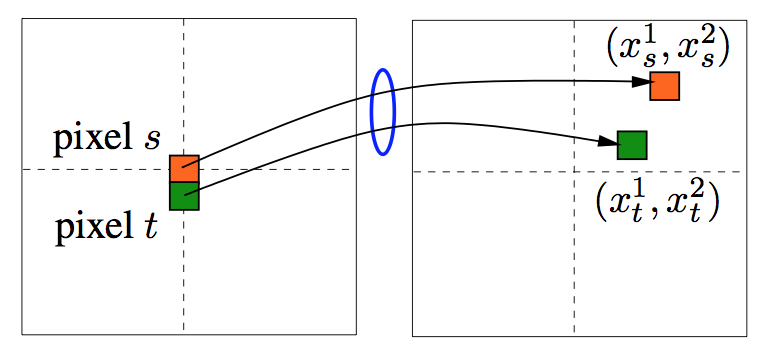
\includegraphics[scale = 0.75]{energy.png}
	\caption{Deformation as pairwise MRF}
	\end{figure}
	\subsubsection{Decomposed Model} We propose a model of \emph{Decomposed Model} \cite{kovtun2004image}, representing $x$ and $y$ displacements by two interacting fields, referred as \emph{layers}. Layer $\Phi^1$ denotes $x$ displacement, and $\Phi_2$ denotes $y$ displacement. Thus our configuration is defined as $\mathbf{x} = \{x_{s^i}|s^i\in\Phi^i,\ i = 1,2\}$. Then the unary term is
	\begin{equation}
		\theta_s{x_s} = \frac{\left(I_s^1 - I_{s+(x_{s^1}, x_{s^2})}\right)^2}{2\sigma_I^2}
	\end{equation}
	And the pairwise term is
	\begin{equation}
		\theta_{st}\left(x_s, x_t\right) = \frac{\left(x_s - x_t\right)^2}{2\sigma_x^2},\ (s,t)\in\mathbb{E}
	\end{equation}
	See Fig. 2.
	\begin{figure}[!hb]
	\centering
	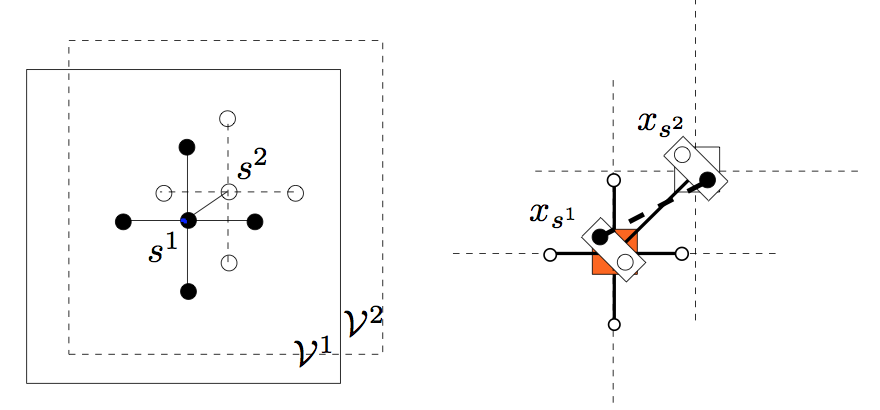
\includegraphics[scale=0.7]{decompose.png}
	\caption{Decomposed Model}
	\end{figure}
	\subsection{Improvements}
		\subsubsection{Block Model}
			If we minimize the energy over all pixels in the image, it will consume a lot of time. So we split the image into blocks to accelerate the compuation. Here we choose block size as 4 pixels. To avoid overfitting, we require the deformation field to be locally affine. As we consider discrete models, we want the deformation field to be described locally by translations. We propose to aggregate pixels into blocks and allow each block to have displacements with a pixel precision. We do not penalize relative displacements of $\pm 1$ pixel in vertical and horizontal directions(see Fig. 3), and completely forbid larger displacements.
			\begin{figure}[!hb]
			\centering
			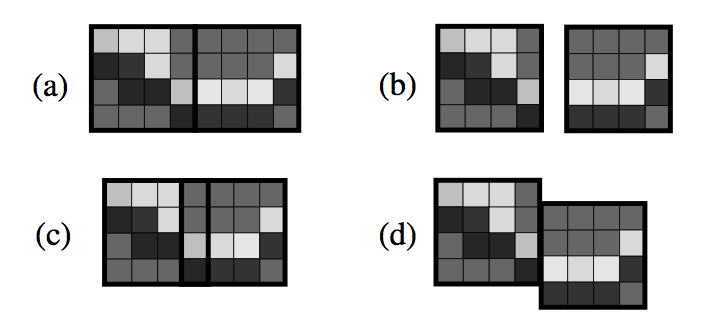
\includegraphics[scale = 0.85]{block.png}
			\caption{Block Model: (a) two neighboring blocks (b)-(d) examples which are not penalized}
			\end{figure}
			So we define the unary term as
			\begin{equation}
				\theta_s(x_s) = \frac{1}{2\sigma_I^2} d(I_s^1, I_{s+(x_{s^1}, x_{s^2})})
			\end{equation}
			where $d(\cdot,\cdot)$ denots for the distance function of two blocks specified in the following. As for the pairwise term, it's defined as
			\begin{equation}
				\theta_{st}(x_s, x_t) = \left\{\begin{array}{ll}
				0 & x_s = x_t \\
				C_r & |x_s - x_t| \leqslant 1\\
				\infty & |x_s - x_t| > 1
				\end{array}\right.
			\end{equation}
			where $\displaystyle{0 < C_r \ll \frac{1}{\sigma_I^2}}$ and we take $C_r = 0.001$ in implementation.
		\subsubsection{Distance of Blocks}
\section{Minimize Energy Function}
	\subsection{ICM}
	Iterative Conditional Modes(ICM)\cite{besag1986} is firstly used to minimize our MRF energy function by us because it can be implemented simply. We will introduce its pipeline and then show the result of this optimization method.
		\subsubsection{ICM Pipeline}

			As for ICM, it traverses the whole label space for each graph nodes. First, we initialize the graph nodes with random labels, then the iteration begins. In each iteration, for every graph node, we try every possible label for it, checking if the energy is smaller than previous configuration. If yes, we update the node with this label. Because we update the labels for nodes only when the energy under current configuration is smaller than previous configuration, it's guaranteed to converge. The pipeline is shown in Algorithm 1.
			\begin{algorithm}
			\caption{Pipeline for ICM}
			\begin{algorithmic}
			\State Initialize each node with a random label
			\While{(Iteration Not Ends)}
				\For{Node $i$ in all graph Nodes}
					\For{Possible Labels for node $i$}
						\If{(Energy is smaller than previous configuration)}
							\State Label for node $i$ := label $j$
						\EndIf
					\EndFor
				\EndFor
				\State Store current configuration
			\EndWhile
			\end{algorithmic}
			\end{algorithm}
        \subsubsection{Define the distance of colors}

        For the color comparison we use
        \begin{equation}
        	F_{\lambda}(c_{1},c_{2}) = {\lambda}^{2} \times \frac{\langle c_{1}-c_{2}, c_{2} \rangle }{ {\left \| c_{2} \right \|}^{2} } + \left(c_{1}-  {\langle c_{1},c_{2} \rangle} \times \frac{c_{2}}{\left \| c_{2} \right \|}^{2}\right)^{2}
        \end{equation}
        We represent color space as $[0,1]^{3}$ and compute color similarity using $F_{\lambda}$ with $\lambda = 0.1 $.\\
        For $d(x,y)$, we use
        \begin{equation}
            d(x,y) = \frac{1}{N} \sum_{k=1}^N  F_{\lambda}\left({x^{i},y^{i}}\right)
        \end{equation}
        where $x^{i}, y^{i}$ are colors of pixels in correspondence. We set $\sigma_{I} = 1 $.


        \subsubsection{Speed up computation}

        We use \textbf{rgb2ind} method in MATLAB to convert RGB color space($256^3$ colors) to 32 colors, which makes computation much more faster as for the computation of color distance. What's more, We use the mix-compile of MATLAB and Java to maintain a Java hashtable, containing $\left(c_{1},c_{2},d(c_{1},c_{2})\right)$. In each computing, our method searches the hashtable first. If the table has the tuple$(c_{1},c_{2})$, the hashtable returns the $d(c_{1},c_{2})$. If not, the programming calculates the distance $d(c_{1},c_{2})$, depending on the definition and saves $\left(c_{1},c_{2},d(c_{1},c_{2})\right)$.

		\subsubsection{Result}
		We use the human face emotion change to show our result(Fig. 4).
		\begin{figure}[!ht]
		\centering
		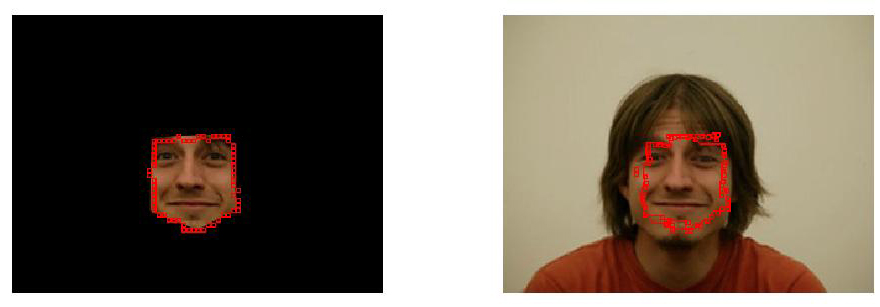
\includegraphics[scale=0.4]{../Result/new-face3.jpg}
		\caption{Result of ICM. Left: the template face. Right: the target face}
		\end{figure}
		We only show the blocks on both template face and target face on the boundary because it will cover the whole face if all blocks are shown. We can see from the result that the deformation of human faces is modeled very well and accurate under the circumstance where the emotion doesn't change too much. Because we restrict that neighboring blocks can't move apart too much, we can model small deformation very well. And since ICM searches for the whold label space and only updates labels when MRF energy is smaller, it's guaranteed to converge.\\
		However, ICM has some shortages. First, it runs very slow. In our experiment\footnote{Intel Core i7 2.7GHz, 8GB DDR3 RAM}, it takes about 30 minutes to compute the deformation for the image shown in Fig. 4, which has 335 blocks. In the future, it will much faster if we use parallel computing because we find that only a single core of CPU is utilized during the computation. Second, if may fall into local minimum.

	\subsection{TRW-S}
		\subsubsection{TRW-S\cite{Chaohui2013}}
        The tree-reweighted message passing (TRW) techniques\cite{kolmogorov2006convergent}, which approach the solution to MRF-LP via a dual problem defined by a convex combination of trees.\\
        A sequential message passing scheme (known as TRW-S) was proposed in this method. It updates messages in a sequential order instead of a parallel order used in TRW-E and TRW-T, which makes the lower bound will not decrease in TRW-S.\\
        Regarding the convergence, TRW-S will attain a point that satisfies a condition referred to as weak tree agreement and the lower bound will not change any more since then.\\
        Regarding the optimality, TRW-S cannot guarantee the global maximum of the lower bound in general.
		\subsubsection{Result}
        In this project, we respect the TRW-S code in \cite{shekhovtsov2008efficient}. The result are shown as Fig. 5.
        \begin{figure}[!ht]
        \centering
        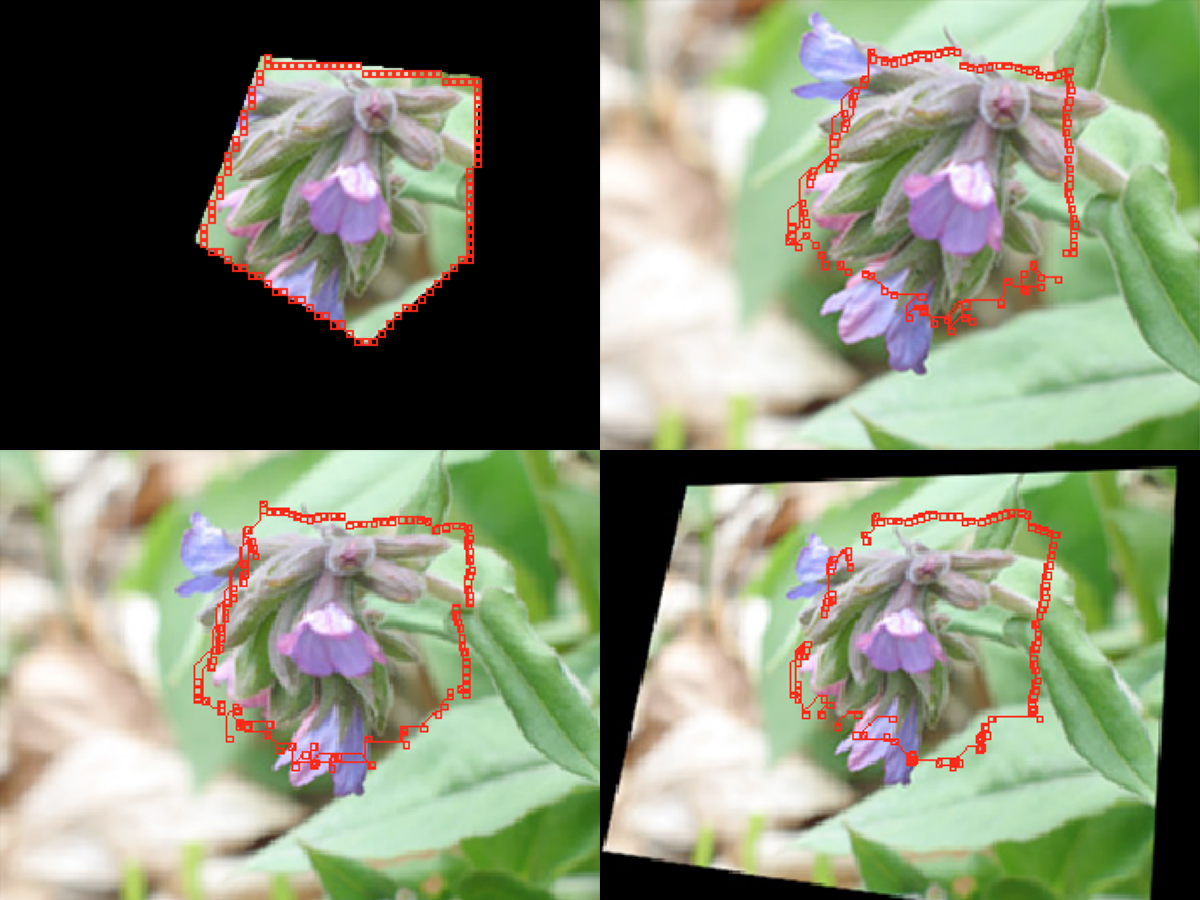
\includegraphics[scale=0.2]{showPlant.jpg}
        \caption{TRW-S Results for the plant image. Top-left: the template image; All others: deformed template blocks on target images.}
        \end{figure}
        And we also do some experiments on brain images, which is widely used in the medical field, which are shown as Fig. 6.
        \begin{figure}[!ht]
        \centering
        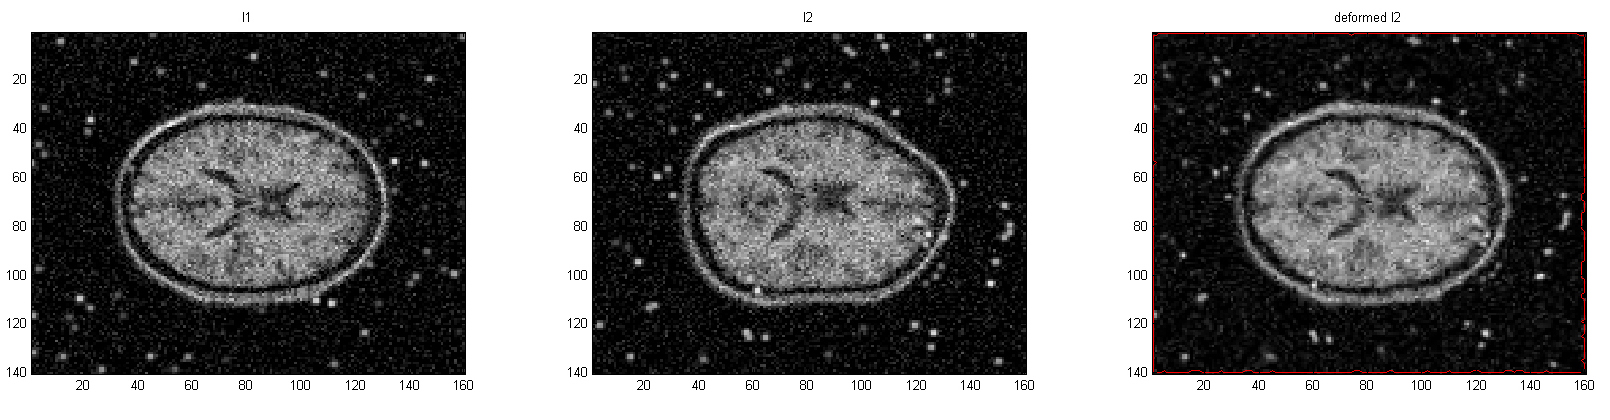
\includegraphics[scale=0.25]{showBrain.jpg}
        \caption{TRW-S Results for the brain image. Left: template brain image; Middle: target image; Right: deformed target image onto template image.}
        \end{figure}
        Our algorithm could also be used for face morphing. Given two images, one of which as template, the other as target, we could obtain the output as the intermediate image as the morphing between two images. We use 3 images and do our experiment for twice, we get two intermediate images as the morphing. The result can be seen in Fig. 7.
        \begin{figure}[!ht]
        \centering
        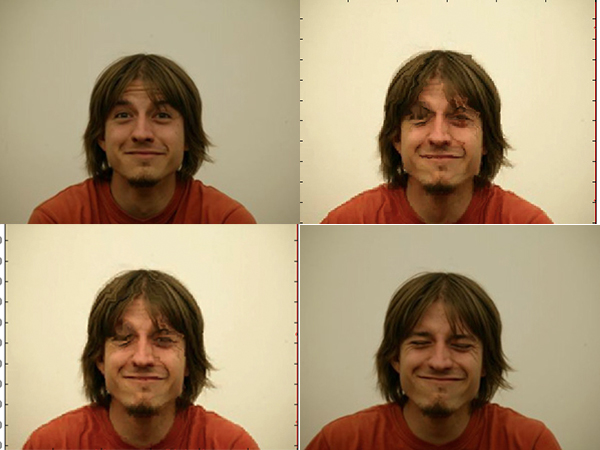
\includegraphics[scale=0.5]{faceMorph.jpg}
        \caption{TRW-S Results for face morphing. Top-left: the template image; Botton-right: the target image; The other two: Intermediate images as face morphing.}
        \end{figure}
        As seen in the result, eyes of the figure in the image are a little opened in the morphing image, compared with the widely opened eyes in the template image and completely closed eyes in the target image. However, because we only use the information from target image and we choose block size as 1 pixel in this experiment, the result has some alias.
\section{Summary and Future Work}
\subsection{Summary}
        In sum, Jason and Jian use the image color information, continuous constrain and MRF algorithm to implement image registration. Jason and Jian construct the two layer model and energy function.\\
        According to MRF algorithm, Jason and Jian implement Iterated Conditional Modes to search fragment and its found deformations superimposed, in addition  also refer author's paper and tree-reweighted message passing algorithm to complete the face morphing. \\


\subsection{Future Work}
        There are two improvements could be done in the next work .\\
        \begin{itemize}
          \item
          The morphing result has some blur in detail. We think the solution is adjusting the model's flexibility parameter $c_{r}$.
          \item
          If we combine the geometry information such as face mesh, the result maybe more accurate.
     
       \end{itemize}
        
        
        
        
\phantomsection
\bibliography{tex}

\end{document}
